\section{Objektdetektoren}

Ein Anwendungsgebiet des \textit{Deep Learnings} beschreiben die Objektdetektoren, die im \textit{Smart Warehouse} Szenario zur Lokalisierung und Klassifizierung von Bestandsobjekten genutzt werden. Im folgenden Kapitel soll demnach der Grundbaustein von Objektdetektoren, das \textit{Convolutional Neural Network}, zunächst genauer betrachtet werden, bevor auf die zwei gängigsten Objektdetektoren, der \textit{Single Shot MultiBox Detector} und der \textit{You Only Look Once} Ansatz eingegangen wird. Es gibt eine weitere Objektdetektor-Familie, die der \textit{Regional Convolutional Neural Networks}. Darunter fallen Architekturen wie \textit{Faster R-CNN} oder \textit{Mask R-CNN}, der sogar eine Segmentierung von Objekten ermöglicht. Auf Grundlage des jetzigen Forschungsstandes ist jedoch bekannt, dass Objektdetektoren der R-CNN Familie nicht performant genug sind, um Echtzeitbedingungen zu erfüllen (siehe Abbildung \ref{result}). Deshalb werden Objektdetektoren dieser Klasse nicht innerhalb dieser Arbeit zusätzlich behandelt.

\subsection*{Convolutional Neural Networks}

Ein CNN besteht aus zwei grundlegenden Bausteinen, den sogenannten \textit{Convolutional Layern} und \textit{Pooling Layern}.

Ein Convolutional Layer zeichnen sich unter anderem dadurch aus, dass jede LTU dieser Schicht nicht mit allen vorherigen LTUs der vorgegangenen Schicht verbunden ist, sondern nur mit einer festen, beschränkten Anzahl. Es ist also kein vollständig verbundenes neuronales Netz. Dies macht es möglich, dass auch große Bilder klassifiziert werden können, ohne dass die Anzahl an nötigen Verbindungen im ANN unüberschaubar groß wächst. Die folgenden LTUs der zweiten Schicht sind ebenfalls wiederum nur mit einem Ausschnitt vorangegangener Neuronen verbunden und fassen die erkannten, kleinteiligen Merkmale der ersten Schicht zu übergeordneten, zusammengesetzten und komplexeren Merkmalen zusammen \cite{AurelienGeron.2018}.

Um allerdings Convolutional Layer genauer zu verstehen, ist anstelle einer eindimensionalen Darstellung eines Layers eine dreidimensionale Darstellung besser geeignet.

Zunächst kann ein zweidimensionale Bild als Matrix dargestellt werden, bei der jedes Element der Matrix den Grauwert eines Pixels zwischen 0 und 255 trägt. Die dadurch entstandene zweidimensionale Schicht bildet den Input-Layer mit einer LTU pro Pixel. Anschließend werden auf diese Schicht mehrere Filter angewandt, die die Gewichte des CNNs tragen und Muster aus dem Bild extrahieren. Die Stellen, die dem Muster ähnlich sind werden verstärkt, während Stellen, die nicht dem Muster entsprechen durch eine Nullgewichtung ausgelöscht werden. In Abbildung \ref{convolutional_layer} ist ein 3x3 Pixel Filter mit dessen Anwendung dargestellt. Ein Filter besitzt die Größe des künstlichen Wahrnehmungsfeldes einer LTU \cite{AurelienGeron.2018}.

\begin{figure}
	\begin{minipage}[b]{.55\linewidth} % [b] => Ausrichtung an \caption
		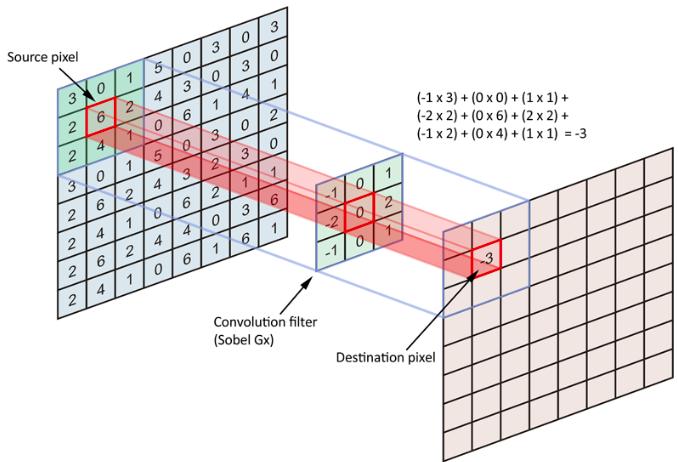
\includegraphics[width=\linewidth]{Bilder/convolutional_layer.png}
		\caption[Convolutional Layer]{Convolutional Layer \cite{DaphneCornelisse.20180424}}
		\label{convolutional_layer}
	\end{minipage}
	\hspace{.05\linewidth}% Abstand zwischen Bilder
	\begin{minipage}[b]{.4\linewidth} % [b] => Ausrichtung an \caption
		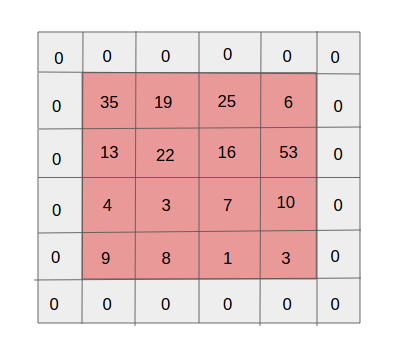
\includegraphics[width=\linewidth]{Bilder/zero_padding.png}
		\caption[Zero-Padding]{Zero-Padding \cite{AbhineetSaxena.20160629}}
		\label{zero_padding}
	\end{minipage}
\end{figure}

Ein Filter wird dazu verwendet, jeden Pixel der Eingabeschicht auf die folgende Schicht abzubilden. Um keine Informationen zu verlieren und den Filter ebenso auf Randbereich anwendbar zu machen, wird oft ein sogenanntes \textit{Zero-Padding} auf eine Schicht angewandt, bei dem die Randbereiche mit LTUs des Wertes 0 aufgefüllt werden (siehe Abbildung \ref{zero_padding}) \cite{AurelienGeron.2018}.

Falls eine gleich große folgende Schicht gewünscht ist, wird eine Schrittweite (engl.: \textit{stride}) von 1 gewählt. Dies dient vor allem dazu kleinere Strukturen noch zu erkennen. Der Filter wird von einem Pixel zum direkt benachbarten Pixel bewegt und angewandt. In tieferen, fortgeschritteneren Schichten kann die Schrittweite auch größer als 1 gewählt werden, da hier bereits nach dem Anwenden mehrerer Filter feinere Muster erkannt wurden und diese nun zu größeren zusammengesetzt werden. Dabei verkleinert sich die resultierende Schicht \cite{AurelienGeron.2018}.

Das Ergebnis der Anwendung eines Filters wird als \textit{Feature-Map} bezeichnet. Da mehrere Filter auf die gleiche Schicht angewandt werden, entstehen ebenso mehrere Feature Maps der Schicht. Werden diese Feature Maps übereinander gelagert vorgestellt, so entsteht der dreidimensionale, \glqq faltungsbedingte\grqq{} (engl.: convolutional) Charakter eines Convolutional Layers. Eine Schicht eines Convolutional Layers ist mit den entsprechenden Wahrnehmungsbereichen aller vorhergehenden Feature Maps des vorhergehenden Convolutional Layers verbunden (siehe Abbildung \ref{feature_maps}) \cite{AurelienGeron.2018}.

\begin{figure}[ht]
	\begin{center}
		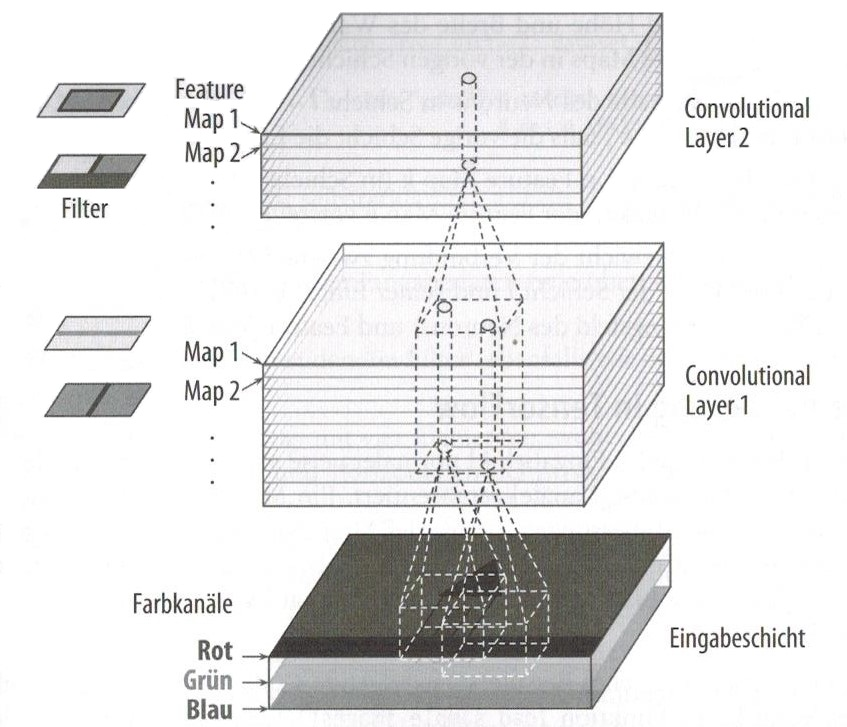
\includegraphics[width=11cm]{Bilder/feature_maps.jpeg} 
		\caption[Feature Maps]{Feature Maps \cite{AurelienGeron.2018}}
		\label{feature_maps}
	\end{center}
\end{figure}

Falls zusätzlich eine Farberkennung gewünscht ist, besitzt der Input Layer für jeden der drei Farbkanäle des RGB-Schemas eine Schicht, die Werte zwischen 0 und 255 in ihren LTUs tragen und den Stärken des Rot-, Grün- und Blaukanals entsprechen \cite{AurelienGeron.2018}.

Der Lernprozess bei der Bilderkennung beruht nun darauf, die optimalsten Filter für die gegebene Aufgabe zu finden und diese zu komplexen Mustern zusammen setzen zu können  \cite{AurelienGeron.2018}.

Der zweite Grundbaustein eines CNN sind Pooling Layer. Ähnlich zu den Convolutional Layern ist auch hier jede LTU nur mit einer begrenzten Anzahl an LTUs des vorhergegangenen Layers verbunden, also nur mit dem lokalen Wahrnehmungsfeld. Der Hauptunterschied liegt aber darin, das keine Filter existieren, die die Eingaben unterschiedlich gewichten und dabei Muster erkennen, sondern stattdessen Aggregatfunktionen wie \textit{MAX()} oder \textit{MEAN()} dazu benutzt werden, um Eingaben zu verkleinern. So wird beispielsweise bei einem MAX-Pooling Layer mit Schrittweite größer als 1 der jeweils größte Wert des lokalen Wahrnehmungsfeld weitergereicht und durch die gewählte Schrittweite das vorherige Ergebnis verkleinert (siehe Abbildung \ref{pooling_layer}), was mit einem Informationsverlust verbunden ist. Dies ist allerdings ein wesentlicher Schritt, um weiter abstrahieren zu können \cite{AurelienGeron.2018}.

\begin{figure}[ht]
	\begin{center}
		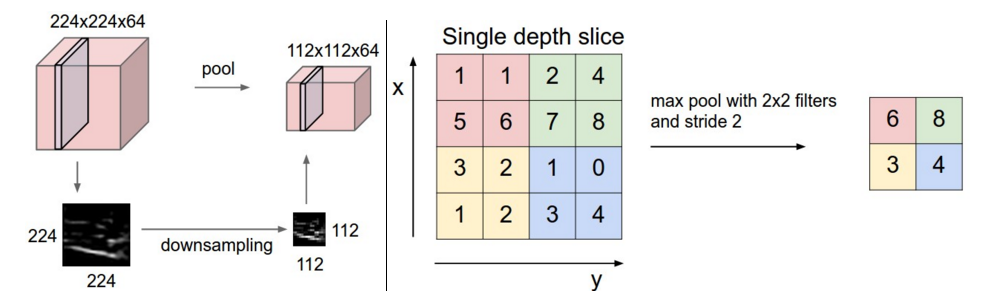
\includegraphics[width=15cm]{Bilder/pooling_layer.png} 
		\caption[Pooling Layer]{Pooling Layer \cite{LeonadroAraujoSantos.2018}}
		\label{pooling_layer}
	\end{center}
\end{figure}

Daneben ist ein Pooling über die Tiefe der Feature Maps möglich, hier bleibt die Größe der resultierenden Feature Maps gleich, die Anzahl verringert sich allerdings \cite{AurelienGeron.2018}.

Nachdem nun beide Grundbausteine eines CNNs genauer erläutert wurden, lassen sich diese nun kombinieren um ein vollständiges CNN zu bauen. Hierbei gibt es unterschiedlichste Architekturen, größtenteils äußerst komplexe. Im Rahmen dieser Arbeit genügt es allerdings die grundlegende Architektur zu erläutern.

Diese beginnt mit einigen Convolutional Layern, die aufeinander folgen und am Ende durch eine ReLU-Funktion nochmals gefiltert und durch ein Pooling Layer abgeschlossen werden. Dies wird je nach Komplexität der zu erkennenden Muster und der Größe der Bilder einige Male wiederholt. Das ursprüngliche Bild wird durch die Pooling Layer zwar immer kleiner, allerdings auch durch die Convolutional Layer immer tiefer. Das CNN schließt mit einem normalen Feed-Forward ANN mit vollständig verbundenen Schichten ab und trifft durch eine Softmax-Funktion eine Klassifikationsaussage des Bildes \cite{AurelienGeron.2018}. 

Diese Architektur ermöglicht ebenso die Wiederverwendbarkeit einzelner Schichten und Gewichtungen für ähnliche Klassifikationsprobleme, bei denen gleiche Muster vorzufinden sind \cite{AurelienGeron.2018}.
